\documentclass[13pt]{article}
\usepackage{amsmath, amsthm, amssymb, graphicx, enumitem, esvect}
\usepackage{graphicx}
\graphicspath{ {./images/} }


% Language setting
% Replace `english' with e.g. `spanish' to change the document language
\usepackage[english]{babel}

% Set page size and margins
% Replace `letterpaper' with `a4paper' for UK/EU standard size
\usepackage[letterpaper,top=2cm,bottom=2cm,left=3cm,right=3cm,marginparwidth=1.75cm]{geometry}

\title{C\&EE 110 Homework 8}
\author{Warren Kim}

\begin{document}
\maketitle

\newpage
\section*{Question 1}
Let $Y$ have probability density function:
$$ f_Y(y) =
\begin{cases}
  \frac{3(\theta^2 - y^2)}{2\theta^3}, & 0 < y < \theta \\
  0, & \textit{elsewhere}
\end{cases} $$
\begin{enumerate}[label=(\alph*)]
\item Show that $\frac{Y}{\theta}$ can be used as a pivitol quantity.
\item Use the pivotal quantity from part (a) to find a $90\%$ confidence limit for $\theta$.
\end{enumerate}

\subsection*{Response}
\begin{enumerate}[label=(\alph*)]
\item
  We are given:
  \begin{align*}
    U &= \frac{Y}{\theta} \implies Y = U\theta = h^{-1}(u) \\
    \frac{d}{du} h^{-1}(u) &= \frac{d}{du} U\theta = \theta
  \end{align*}
  Then, we have:
  \begin{align*}
    f_u(U) &= f_y\left(h^{-1}(u)\right) \left|\frac{d}{du} h^{-1}\right| \\
           &= \frac{3(\theta^2 - \left(u\theta\right)^2)}{2\theta^3} \left|\theta\right| \\
           &= \frac{3\theta^3(1 - u^2)}{2\theta^3} \\
    f_u(U) &= \frac{3(1 - u^2)}{2}
  \end{align*}
  $f_u(U)$ does not depend on $\theta \implies U$ can be used as a pivotal quantity.
  
\item
  \begin{align*}
    0.10 &= \int_0^a f_u(U)du = \int_0^a \frac{3(1 - u^2)}{2} du \\
         &= \frac{3}{2} \int_0^a (1 - u^2) du \\
         &= \frac{1}{2}\left(3u - u^3\right) \bigg|_0^a \\
    a &= 0.067 \\
         \implies \theta &= \frac{Y}{0.067}
  \end{align*}  
\end{enumerate}

\newpage
\section*{Question 2}
The breaking strength of hockey stick shafts made of two different graphite-Kevlar
composites yield the following results (in newtons):
\begin{itemize}
\item Composite A: $487.3 \ 444.5 \ 467.7 \ 456.3 \ 449.7 \ 459.2 \ 478.9 \ 461.5 \ 477.2$
\item Composite B: $488.5 \ 501.2 \ 475.3 \ 467.2 \ 462.5 \ 499.7 \ 470.0 \ 469.5 \ 481.5 \ 485.2
  \ 509.3 \ 479.3 \ 478.3 \ 491.5$
\end{itemize}
Find a $98\%$ confidence interval for the difference between the mean breaking strengths of hockey stick
shafts made of the two materials for two cases:
\begin{enumerate}[label=(\alph*)]
\item The population variances are not necessarily the same.
\item The population variances can be assumed to be similar.
\end{enumerate}

\subsection*{Response}
\begin{enumerate}[label=(\alph*)]
\item
  We are given for $A$:
  \begin{align*}
    s &= 14.238 \\
    s^2 &= 202.718 \\
    n &= 9 \\
    \overline{x} &= 464.7 \\
  \end{align*}
  We are given for $B$:
  \begin{align*}
    s &= 13.942 \\
    s^2 &= 194.383 \\
    n &= 14 \\
    \overline{x} &= 482.786 \\
  \end{align*}
  Then we have:
  \begin{align*}
    v &= \frac{\left( \frac{s_A^2}{n_A} + \frac{s_B^2}{n_B} \right)^2}
        {\frac{ \left( \frac{s_A^2}{n_A} \right)^2 }{n_A - 1} + \frac{ \left( \frac{s_B^2}{n_B} \right)^2 }{n_B - 1}} \\
      &= \frac{\left( \frac{202.718}{9} + \frac{194.38}{14} \right)^2}
        {\frac{ \left( \frac{202.718}{9} \right)^2 }{9 - 1} + \frac{ \left( \frac{194.38}{14} \right)^2 }{14 - 1}} \\
      &= 16.941 \\
    \implies df &= 17
  \end{align*}
  $\alpha = 0.02 \implies t_{17, \ 0.02} = 2.567$. Then,
  \begin{align*}
    (\mu_A - \mu_B) \pm t_{17, \ 0.02} \sqrt{\frac{s_A^2}{n_A} + \frac{s_B^2}{n_B}} \\
    (464.7 - 482.786) \pm 2.567 \sqrt{\frac{202.718}{9} + \frac{194.383}{14}} \\
    [-33.575, -2.597]
  \end{align*}
  
\newpage  
\item
  We have:
  \begin{align*}
    S_p^2 &= \sqrt{\frac{(n_A - 1)S_1^2 + (n_B - 1)S_2^2}{n_1 + n_2 - 2}} \\
          &= \frac{(9 - 1)(202.718) + (14 - 1)(194.383)}{9 + 14 - 2} \\
          &= \frac{4148.717}{21} \\
    S_p^2 &= 197.558 \\
    S_p &= 14.056
  \end{align*}
  Then, 
  \begin{align*}
    \left( \overline{Y}_A - \overline{Y}_B \right) \pm t_{df, \frac{\alpha}{2}}S_P\sqrt{\frac{1}{n_A} + \frac{1}{n_B}} \\
    (464.7 - 482.786) \pm t_{21, 0.02} (14.056) \sqrt{\frac{1}{9} + \frac{1}{14}} \\
    [-33.206, -2.965]
  \end{align*}
\end{enumerate}


\newpage
\section*{Question 3}
The following table shows the results of a uniaxial strength testing for a new steel alloy that
UCLA is developing. The underlying distribution for the strength of this new material is estimated
to be normal. \\
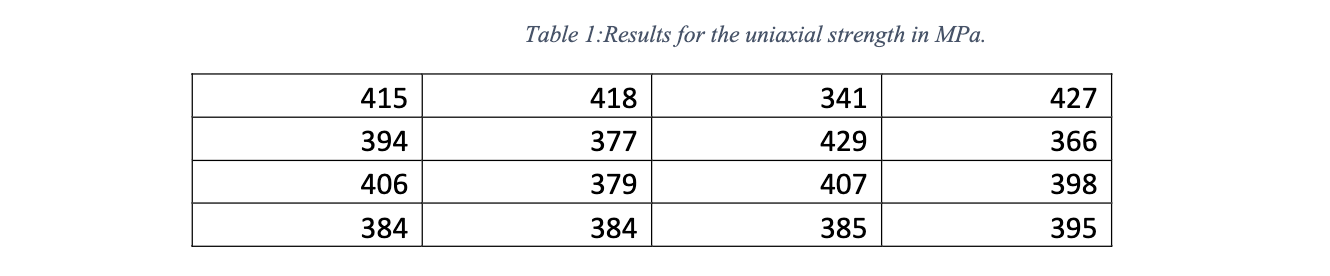
\includegraphics[scale=0.65]{table}
\begin{enumerate}[label=(\alph*)]
\item Obtain the Maximum Likelihood Estimators for the mean and variance of the underlying distribution
  (derive them analytically, showing the complete process).
\item Using the Maximum Likelihood Estimators obtained in part (a), compute the point esimates for the
  mean and variance based on the data shown in Table 1.
\item An alternative version of this material is being developed in parallel, and the objective is to test
  whether a different percentage in carbon can increase the strength of the steel alloy with respect to the
  original formula (part (a), (b)). For this, 45 samples with this alternative recipe are forged and tested,
  obtaining measurements with mean strength of $412.6 [MPa]$ and a standard deviation of $15.5 MPa$.
  \begin{enumerate}[label=(\roman*)]
  \item Set up the null and alternative hypothesis. Is this a two-tailed test or one-tailed test?
  \item Can you conclude that the new recipe effectively increases the strength of the material? Use a
    confidence interval of $\alpha = 0.05$.
  \end{enumerate}
\end{enumerate}

\subsection*{Response}
\begin{enumerate}[label=(\alph*)]
\item We have that the underlying distribution is estimated to be normal. Then, we have $X_1, \ldots, X_n$.
  \begin{align*}
    L(\mu, \sigma^2) &= f(x_1, \ldots, x_n | \mu, \sigma^2) \\
                     &= \prod_{i = 1}^{n} f(x_i | \mu, \sigma^2) \\
                     &= \prod_{i = 1}^{n} \left\{ \frac{1}{\sigma \sqrt{2\pi}}
                       \exp \left[ \frac{-(x_i - \mu)^2}{2\sigma^2} \right]\right\} \\
    L(\mu, \sigma^2) &= \left( \frac{1}{2 \pi \sigma^2} \right)^{\frac{n}{2}}
                       \exp \left[ \frac{-1}{2\sigma^2} \sum_{i = 1}^{n}(x_i - \mu)^2 \right]
  \end{align*}
  Then,
  \[\ln\left[ L(\mu, \sigma^2 \right] =
  -\frac{n}{2}\ln \left(\sigma^2\right)
  - \frac{n}{2}\ln \left(2 \pi \right)
  - \frac{1}{2\sigma^2}\sum\limits_{i = 1}^{n}(x_i - \mu)^2\]
  The $MLE$ of $\mu$ and $\sigma^2$ are values such that $\ln\left[ L(\mu, \sigma^2 \right]$ is a max. So, we have:
  \[\frac{\partial \left\{ \ln \left[ L(\mu, \sigma^2) \right] \right\}}{\partial \mu}
    = \frac{1}{\sigma^2}\sum\limits_{i = 1}^{n}(x_i - \mu)^2\]
  and
  \[\frac{\partial \left\{ \ln \left[ L(\mu, \sigma^2) \right] \right\}}{\partial \sigma^2}
    = -\left( \frac{n}{2} \right) \left( \frac{1}{\sigma^2} \right) +
    \frac{1}{2\sigma^4}\sum\limits_{i = 1}^{n}(x_i - \mu)^2\]
  solving for when the derivatives are 0, we get:
  \[\frac{1}{\sigma^2} \sum\limits_{i = 1}^{n} (x_i - \hat{\mu}) = 0
    \implies \sum\limits_{i = 1}^{n}x_i - n \hat{\mu} = 0
    \implies \hat{\mu} = \frac{1}{n} \sum\limits_{i = 1}^{n}x_i = \overline{x}\]
  and
  \[-\left( \frac{n}{\hat{\sigma}^2} \right) +
    \frac{1}{\hat{\sigma}^4} \sum\limits_{i = 1}^{n}(x_i - \overline{x})^2 = 0
    \implies \hat{\sigma}^2 = \frac{1}{n} \sum\limits_{i = 1}^{n}(x_i - \overline{x})^2\]
  Then, $\overline{x}$ and $\hat{\sigma}^2 = \frac{1}{n} \sum\limits_{i = 1}^{n}(x_i - \overline{x})^2$ are
  $MLE$'s of $\mu$ and $\sigma^2$.
  
\item
  \begin{align*}
    \hat{\mu}_n &= \frac{1}{n}\sum\limits_{i = 1}^{n}x_i = 394.063 \\
    \hat{\sigma}^2 &= \frac{1}{n}\sum\limits_{i = 1}^{n}(x_i - 394.063)^2 = 536.596
  \end{align*}

\item 
  We are given: $\overline{x} = 412.6$ and $s = 15.5$. Then,
  \begin{enumerate}[label=(\roman*)]
  \item
    \begin{align*}
      \textit{Null Hypothesis: } H_0: \hat{\mu}_n \leq 394.063 \\
      \textit{Alternative Hypothesis: } H_a: \hat{\mu}_n > 394.063
    \end{align*}
    This is a one tailed test because we are testing for an increase in the parameter.
  \item We reject the $H_0$ if $z > z_\alpha$:
    \begin{align*}
      z &= \frac{\overline{x} - \mu_0}{\frac{s}{\sqrt{n}}} \\
        &= \frac{412.6 - 394.063}{\frac{15.5}{\sqrt{45}}} \\
      z &= 8.02
    \end{align*}
    $\textit{A cumulative area of } 0.95 \implies z_\alpha = 1.64$. Then,
    \[z = 8.02 > 1.64 = z_\alpha \implies \textit{reject } H_0\]
    Thus, we reject $H_0$.
  \end{enumerate}
\end{enumerate}
\end{document}

%%% Local Variables:
%%% mode: latex
%%% TeX-master: t
%%% End:
